\documentclass[tikz]{standalone}

\usepackage{circuitikz}

\begin{document}
	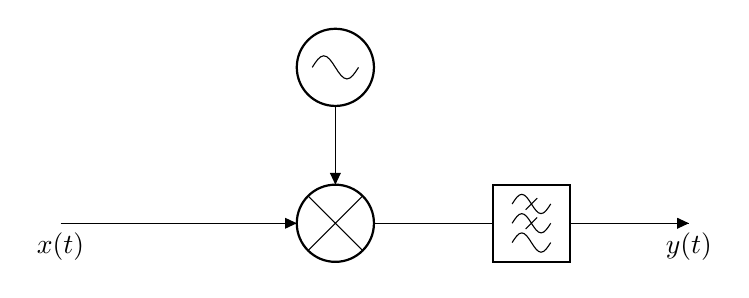
\begin{tikzpicture}
		\draw (0,0) node[below]{$x(t)$} to[short] (3,0)
            node[mixer, anchor=west](mixer){} node[inputarrow]{};
        \draw (mixer.north) node[inputarrow, rotate=-90]{} to[short] ++(0,1) node[oscillator, anchor=south]{};
        \draw (mixer.east) to[lowpass] ++(4,0) node[inputarrow]{} node[below]{$y(t)$};
	\end{tikzpicture}
\end{document}